

Data was queried using USGS Earthquake Catalog:
\url{https://earthquake.usgs.gov/earthquakes/search/} to select all
recorded earthquakes of magnitude 4.5 and above with the following query
parameters:

\begin{itemize}
\tightlist
\item
  latitude 35.4 - 41.2
\item
  longitude 137.5 - 145.2
\item
  Timeframe(UTC): 2011-03-11 00:00:00 - 1965-01-01 00:00:00
\end{itemize}

The data was stored locally in a .csv file named \texttt{earthquakes}.

The organization also has an package called \texttt{rcomcat} to query
data directly into \texttt{R}, but its version was not compatible at the
time of this thesis.

\hypertarget{data-preprocessing}{%
\subsection{Data Preprocessing}\label{data-preprocessing}}

\begin{Shaded}
\begin{Highlighting}[]
\CommentTok{\# load the data }
\NormalTok{earthquakes\_full }\OtherTok{\textless{}{-}} \FunctionTok{read.csv}\NormalTok{(}\StringTok{"data/earthquakes.csv"}\NormalTok{)}

\CommentTok{\# fsbset data to include observations from January 1, 1965 to}
\CommentTok{\#  just before the Greak Quake of March 11, 2011}
\NormalTok{earthquakes\_subset }\OtherTok{\textless{}{-}}\NormalTok{ earthquakes\_full[}\FunctionTok{which}\NormalTok{(earthquakes\_full}\SpecialCharTok{$}\NormalTok{time }\SpecialCharTok{\textgreater{}=} \StringTok{"1965{-}01{-}26T23:47:37.120Z"} \SpecialCharTok{\&}\NormalTok{                                                                      earthquakes\_full}\SpecialCharTok{$}\NormalTok{time }\SpecialCharTok{\textless{}=} \StringTok{"2011{-}03{-}11T05:44:24.120Z"}\NormalTok{),]}
  
\CommentTok{\# fine{-}tune the geographic area of the model}
\NormalTok{earthquakes\_subset }\OtherTok{\textless{}{-}}\NormalTok{ earthquakes\_subset[}\FunctionTok{which}\NormalTok{(earthquakes\_subset}\SpecialCharTok{$}\NormalTok{latitude }\SpecialCharTok{\textgreater{}} \FloatTok{35.72} \SpecialCharTok{\&}
\NormalTok{                                               earthquakes\_subset}\SpecialCharTok{$}\NormalTok{latitude }\SpecialCharTok{\textless{}} \FloatTok{40.82} \SpecialCharTok{\&}
\NormalTok{                                               earthquakes\_subset}\SpecialCharTok{$}\NormalTok{longitude }\SpecialCharTok{\textgreater{}} \FloatTok{139.37} \SpecialCharTok{\&}
\NormalTok{                                               earthquakes\_subset}\SpecialCharTok{$}\NormalTok{longitude }\SpecialCharTok{\textless{}} \FloatTok{143.37}\NormalTok{),]}

\CommentTok{\# data frame of magnitudes (rounded to .1) and relative frequencies}
\NormalTok{eq }\OtherTok{\textless{}{-}} \FunctionTok{data.frame}\NormalTok{(}\FunctionTok{table}\NormalTok{(}\FunctionTok{round}\NormalTok{(earthquakes\_subset}\SpecialCharTok{$}\NormalTok{mag, }\DecValTok{1}\NormalTok{)) ) }\SpecialCharTok{\%\textgreater{}\%} 
                 \FunctionTok{rename}\NormalTok{(}\AttributeTok{mag =}\NormalTok{ Var1,}
                       \AttributeTok{freq =}\NormalTok{ Freq) }\SpecialCharTok{\%\textgreater{}\%} 
                 \FunctionTok{mutate}\NormalTok{(}\AttributeTok{mag =} \FunctionTok{as.numeric}\NormalTok{(}\FunctionTok{as.character}\NormalTok{(mag))) }\SpecialCharTok{\%\textgreater{}\%} \CommentTok{\#change to numeric rather than factors}
                 \FunctionTok{mutate}\NormalTok{(}\AttributeTok{freq =}\NormalTok{ freq}\SpecialCharTok{/}\NormalTok{(}\DecValTok{2011{-}1965}\NormalTok{))      }\CommentTok{\#AVERAGE annual frequencies over the 46{-}year span}

\CommentTok{\# create a new variable representing the frequency of earthquakes of AT LEAST that magnitude}
\ControlFlowTok{for}\NormalTok{(i }\ControlFlowTok{in} \DecValTok{1}\SpecialCharTok{:}\FunctionTok{as.numeric}\NormalTok{(}\FunctionTok{count}\NormalTok{(eq)))\{}
\NormalTok{  eq}\SpecialCharTok{$}\NormalTok{freqc[i] }\OtherTok{\textless{}{-}} \FunctionTok{sum}\NormalTok{( eq}\SpecialCharTok{$}\NormalTok{freq[}\FunctionTok{c}\NormalTok{(i}\SpecialCharTok{:}\FunctionTok{as.numeric}\NormalTok{(}\FunctionTok{count}\NormalTok{(eq)))] )}
\NormalTok{\}}

\CommentTok{\# data set to be worked with on with cumulative frequencies on the log scale}
\NormalTok{eq\_log }\OtherTok{\textless{}{-}}\NormalTok{ eq }\SpecialCharTok{\%\textgreater{}\%} \FunctionTok{mutate}\NormalTok{(}\AttributeTok{freqc =} \FunctionTok{log10}\NormalTok{(freqc))}
\end{Highlighting}
\end{Shaded}

\hypertarget{frequency-of-earthquakes}{%
\subsection{Frequency of Earthquakes}\label{frequency-of-earthquakes}}

Plots of average annual earthquake frequencies over the 46-year span

\begin{Shaded}
\begin{Highlighting}[]
\CommentTok{\#{-}{-}{-}frequencies of each magnitude on the standard scale}
\FunctionTok{ggplot}\NormalTok{(eq, }\FunctionTok{aes}\NormalTok{(}\AttributeTok{x =}\NormalTok{ mag, }\AttributeTok{y =}\NormalTok{ freqc)) }\SpecialCharTok{+}
  \FunctionTok{geom\_point}\NormalTok{(}\AttributeTok{size =} \DecValTok{4}\NormalTok{, }\AttributeTok{shape =} \DecValTok{17}\NormalTok{ ) }\SpecialCharTok{+}
    \FunctionTok{theme\_minimal}\NormalTok{() }\SpecialCharTok{+}
    \FunctionTok{labs}\NormalTok{(}\AttributeTok{x =} \StringTok{"Magnitude"}\NormalTok{,}
       \AttributeTok{y =} \StringTok{"Annual Frequency of At Least this Magnitude"}\NormalTok{,}
       \AttributeTok{title =} \StringTok{"Annual Earthquake Frequency near Tohoku, Japan"}\NormalTok{ ) }\SpecialCharTok{+}
  \FunctionTok{ylim}\NormalTok{(}\DecValTok{0}\NormalTok{,}\DecValTok{50}\NormalTok{)}
\end{Highlighting}
\end{Shaded}

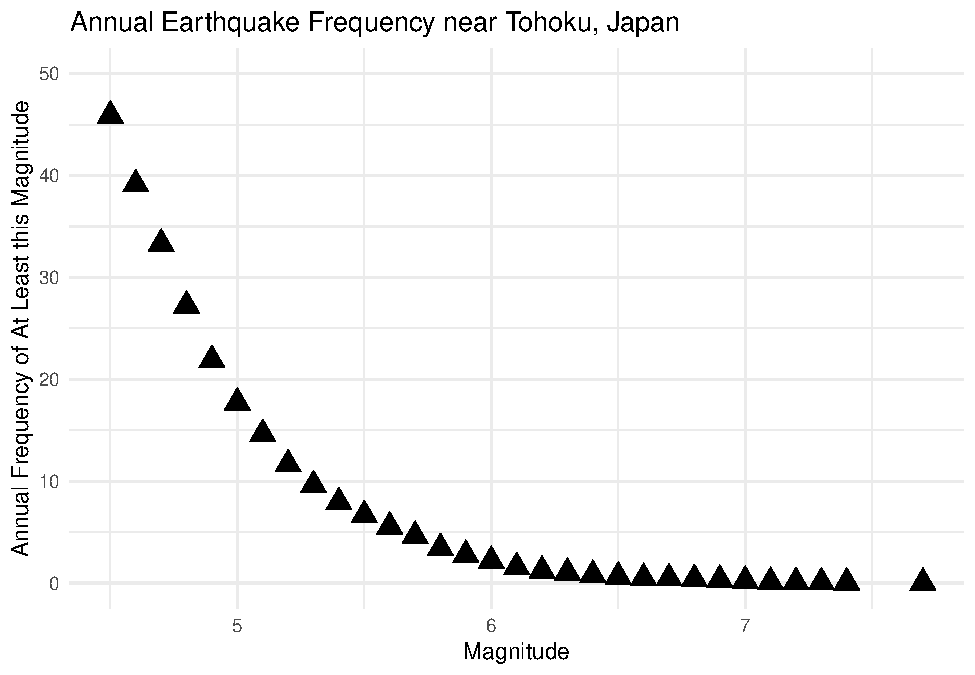
\includegraphics{earthquakes_files/figure-latex/unnamed-chunk-4-1.pdf}

\begin{Shaded}
\begin{Highlighting}[]
\CommentTok{\#{-}{-}{-}frequencies on the logarithmic scale}
\FunctionTok{ggplot}\NormalTok{(eq, }\FunctionTok{aes}\NormalTok{(}\AttributeTok{x =}\NormalTok{ mag, }\AttributeTok{y =}\NormalTok{ freqc)) }\SpecialCharTok{+}
  \FunctionTok{geom\_point}\NormalTok{(}\AttributeTok{size =} \DecValTok{4}\NormalTok{, }\AttributeTok{shape =} \DecValTok{17}\NormalTok{ ) }\SpecialCharTok{+}
  \FunctionTok{theme\_minimal}\NormalTok{() }\SpecialCharTok{+}
  \FunctionTok{scale\_y\_log10}\NormalTok{(}\AttributeTok{limits =} \FunctionTok{c}\NormalTok{(.}\DecValTok{001}\NormalTok{,}\DecValTok{100}\NormalTok{)) }\SpecialCharTok{+}
  \FunctionTok{scale\_x\_log10}\NormalTok{(}\AttributeTok{limits =} \FunctionTok{c}\NormalTok{(}\FloatTok{4.5}\NormalTok{,}\DecValTok{10}\NormalTok{)) }\SpecialCharTok{+}
  \FunctionTok{labs}\NormalTok{(}\AttributeTok{x =} \StringTok{"Magnitude"}\NormalTok{,}
       \AttributeTok{y =} \StringTok{"Annual Frequency of At Least this Magnitude"}\NormalTok{,}
       \AttributeTok{title =} \StringTok{"Annual Earthquake Frequency near Tohoku, Japan {-} Logarithmic Scale"}\NormalTok{ )}
\end{Highlighting}
\end{Shaded}

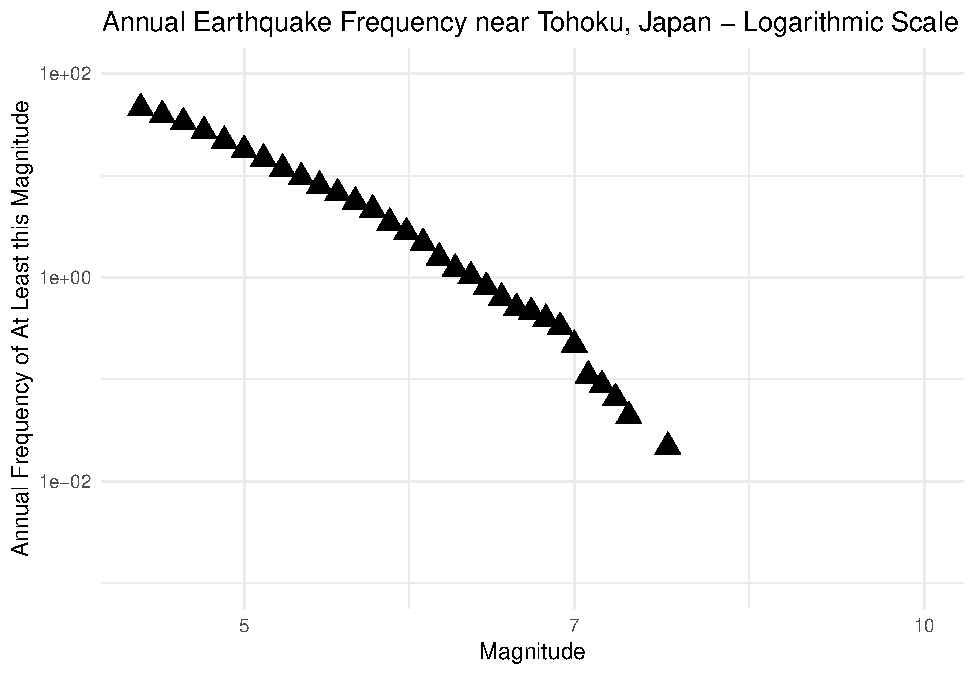
\includegraphics{earthquakes_files/figure-latex/unnamed-chunk-4-2.pdf}

\begin{Shaded}
\begin{Highlighting}[]
\CommentTok{\#{-}{-}{-}frequencies on the logarithmic scale, first order polynomial}
\FunctionTok{ggplot}\NormalTok{(eq, }\FunctionTok{aes}\NormalTok{(}\AttributeTok{x =}\NormalTok{ mag, }\AttributeTok{y =}\NormalTok{ freqc)) }\SpecialCharTok{+}
  \FunctionTok{geom\_point}\NormalTok{(}\AttributeTok{size =} \DecValTok{4}\NormalTok{, }\AttributeTok{shape =} \DecValTok{17}\NormalTok{ ) }\SpecialCharTok{+}
  \FunctionTok{theme\_minimal}\NormalTok{() }\SpecialCharTok{+}
  \FunctionTok{scale\_y\_log10}\NormalTok{(}\AttributeTok{limits =} \FunctionTok{c}\NormalTok{(.}\DecValTok{001}\NormalTok{,}\DecValTok{100}\NormalTok{)) }\SpecialCharTok{+}
  \FunctionTok{scale\_x\_log10}\NormalTok{(}\AttributeTok{limits =} \FunctionTok{c}\NormalTok{(}\FloatTok{4.5}\NormalTok{,}\DecValTok{10}\NormalTok{)) }\SpecialCharTok{+}
  \FunctionTok{labs}\NormalTok{(}\AttributeTok{x =} \StringTok{"Magnitude"}\NormalTok{,}
       \AttributeTok{y =} \StringTok{"Annual Frequency of At Least this Magnitude"}\NormalTok{,}
       \AttributeTok{title =} \StringTok{"Annual Earthquake Frequency near Tohoku, Japan {-} Logarithmic Scale"}\NormalTok{,}
       \AttributeTok{subtitle =} \StringTok{"Linear Model with Minimized Capacity"}\NormalTok{) }\SpecialCharTok{+}
  \FunctionTok{stat\_smooth}\NormalTok{(}\AttributeTok{method =}\NormalTok{ lm,}
              \AttributeTok{formula =}\NormalTok{ y }\SpecialCharTok{\textasciitilde{}} \FunctionTok{poly}\NormalTok{(x,}\DecValTok{1}\NormalTok{),}
              \AttributeTok{fullrange =}\NormalTok{ T)}
\end{Highlighting}
\end{Shaded}

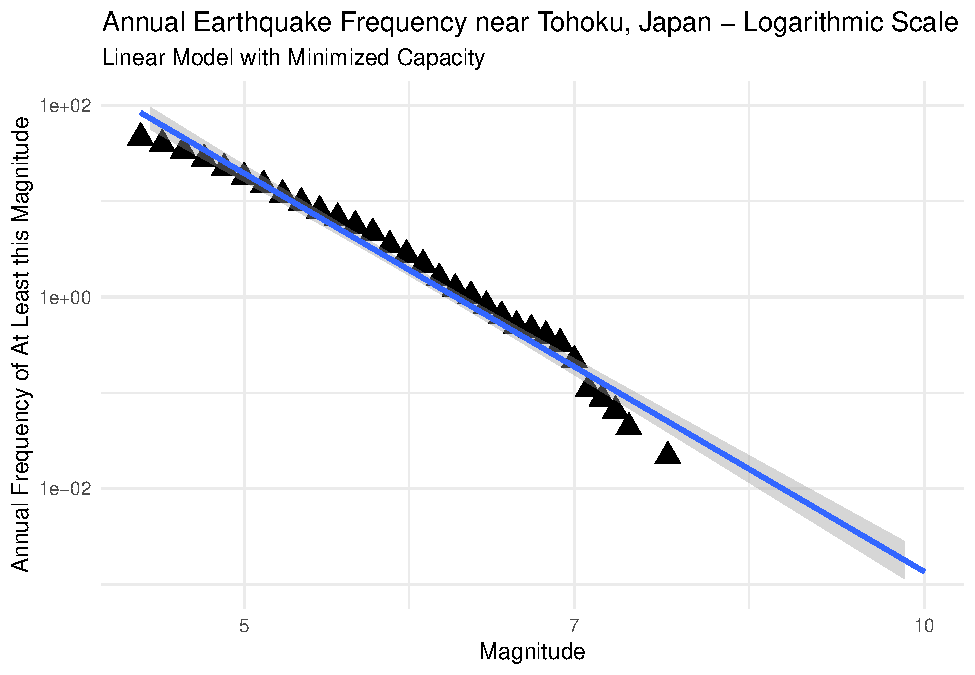
\includegraphics{earthquakes_files/figure-latex/unnamed-chunk-4-3.pdf}

\begin{Shaded}
\begin{Highlighting}[]
\CommentTok{\#{-}{-}{-}frequencies on the logarithmic scale, second order polynomial}
\FunctionTok{ggplot}\NormalTok{(eq, }\FunctionTok{aes}\NormalTok{(}\AttributeTok{x =}\NormalTok{ mag, }\AttributeTok{y =}\NormalTok{ freqc)) }\SpecialCharTok{+}
  \FunctionTok{geom\_point}\NormalTok{(}\AttributeTok{size =} \DecValTok{4}\NormalTok{, }\AttributeTok{shape =} \DecValTok{17}\NormalTok{ ) }\SpecialCharTok{+}
  \FunctionTok{theme\_minimal}\NormalTok{() }\SpecialCharTok{+}
  \FunctionTok{scale\_y\_log10}\NormalTok{(}\AttributeTok{limits =} \FunctionTok{c}\NormalTok{(.}\DecValTok{001}\NormalTok{,}\DecValTok{100}\NormalTok{)) }\SpecialCharTok{+}
  \FunctionTok{scale\_x\_log10}\NormalTok{(}\AttributeTok{limits =} \FunctionTok{c}\NormalTok{(}\FloatTok{4.5}\NormalTok{,}\DecValTok{10}\NormalTok{)) }\SpecialCharTok{+}
  \FunctionTok{labs}\NormalTok{(}\AttributeTok{x =} \StringTok{"Magnitude"}\NormalTok{,}
       \AttributeTok{y =} \StringTok{"Annual Frequency of At Least this Magnitude"}\NormalTok{,}
       \AttributeTok{title =} \StringTok{"Annual Earthquake Frequency near Tohoku, Japan {-} Logarithmic Scale"}\NormalTok{,}
       \AttributeTok{subtitle =} \StringTok{"Linear Model with Second Order Polynomial"}\NormalTok{) }\SpecialCharTok{+}
  \FunctionTok{stat\_smooth}\NormalTok{(}\AttributeTok{method =}\NormalTok{ lm,}
              \AttributeTok{formula =}\NormalTok{ y }\SpecialCharTok{\textasciitilde{}} \FunctionTok{poly}\NormalTok{(x,}\DecValTok{2}\NormalTok{),}
              \AttributeTok{fullrange =}\NormalTok{ T)}
\end{Highlighting}
\end{Shaded}

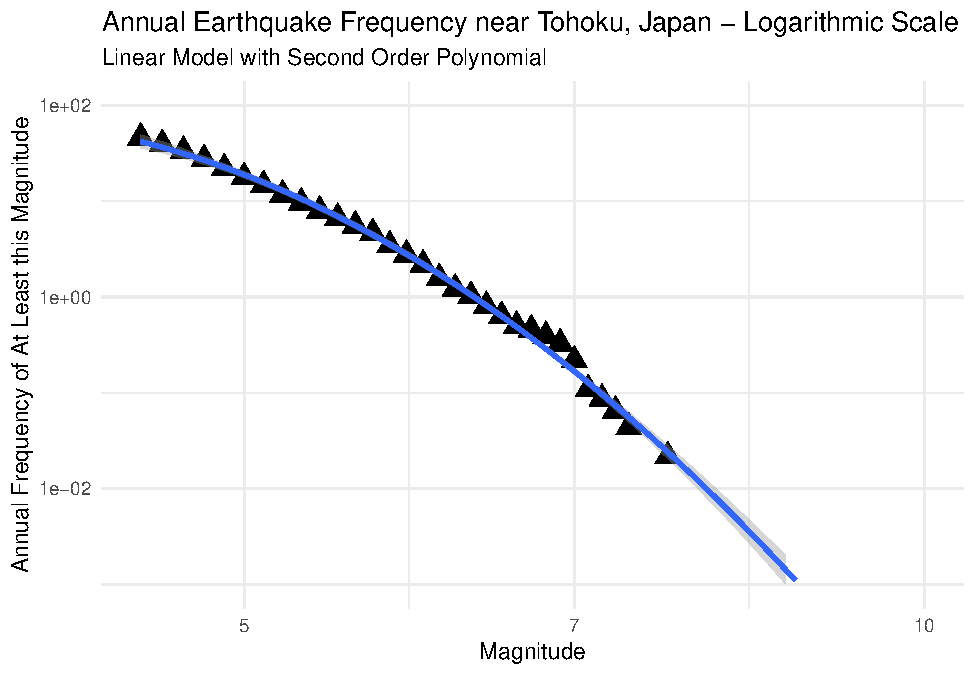
\includegraphics{earthquakes_files/figure-latex/unnamed-chunk-4-4.pdf}

\begin{Shaded}
\begin{Highlighting}[]
\CommentTok{\#{-}{-}{-}frequencies on the logarithmic scale, third order polynomial}
\FunctionTok{ggplot}\NormalTok{(eq, }\FunctionTok{aes}\NormalTok{(}\AttributeTok{x =}\NormalTok{ mag, }\AttributeTok{y =}\NormalTok{ freqc)) }\SpecialCharTok{+}
  \FunctionTok{geom\_point}\NormalTok{(}\AttributeTok{size =} \DecValTok{4}\NormalTok{, }\AttributeTok{shape =} \DecValTok{17}\NormalTok{ ) }\SpecialCharTok{+}
  \FunctionTok{theme\_minimal}\NormalTok{() }\SpecialCharTok{+}
  \FunctionTok{scale\_y\_log10}\NormalTok{(}\AttributeTok{limits =} \FunctionTok{c}\NormalTok{(.}\DecValTok{001}\NormalTok{,}\DecValTok{100}\NormalTok{)) }\SpecialCharTok{+}
  \FunctionTok{scale\_x\_log10}\NormalTok{(}\AttributeTok{limits =} \FunctionTok{c}\NormalTok{(}\FloatTok{4.5}\NormalTok{,}\DecValTok{10}\NormalTok{)) }\SpecialCharTok{+}
  \FunctionTok{labs}\NormalTok{(}\AttributeTok{x =} \StringTok{"Magnitude"}\NormalTok{,}
       \AttributeTok{y =} \StringTok{"Annual Frequency of At Least this Magnitude"}\NormalTok{,}
       \AttributeTok{title =} \StringTok{"Annual Earthquake Frequency near Tohoku, Japan {-} Logarithmic Scale"}\NormalTok{,}
       \AttributeTok{subtitle =} \StringTok{"Linear Model with Third Order Polynomial"}\NormalTok{) }\SpecialCharTok{+}
  \FunctionTok{stat\_smooth}\NormalTok{(}\AttributeTok{method =}\NormalTok{ lm,}
              \AttributeTok{formula =}\NormalTok{ y }\SpecialCharTok{\textasciitilde{}} \FunctionTok{poly}\NormalTok{(x,}\DecValTok{3}\NormalTok{),}
              \AttributeTok{fullrange =}\NormalTok{ T)}
\end{Highlighting}
\end{Shaded}

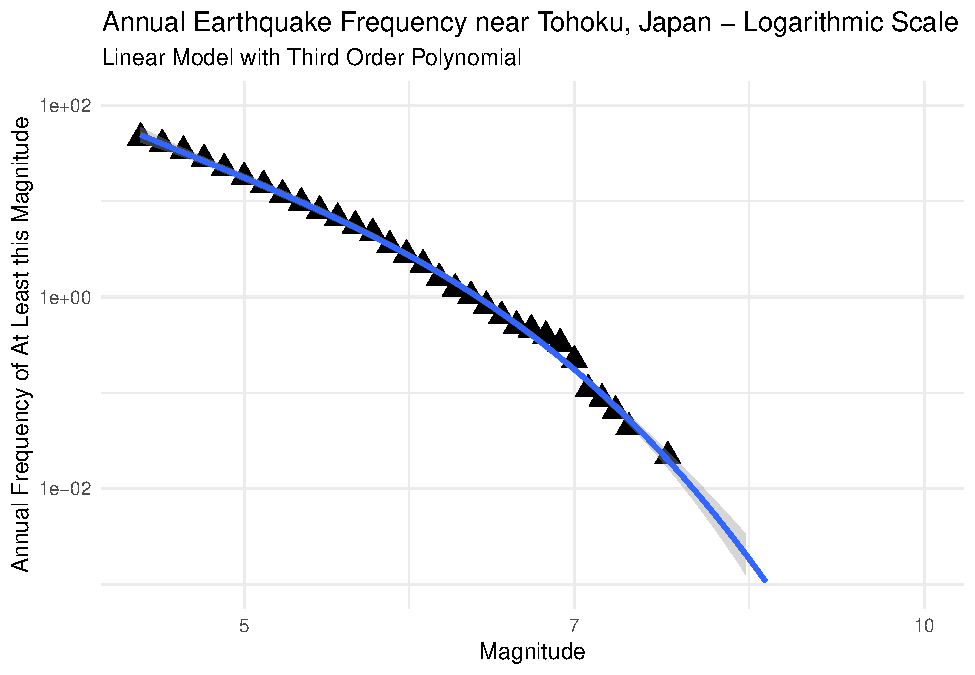
\includegraphics{earthquakes_files/figure-latex/unnamed-chunk-4-5.pdf}

\hypertarget{linear-models-of-the-data}{%
\subsection{Linear models of the data}\label{linear-models-of-the-data}}

Calculation of a single variable linear model on the logarithmic scale
with no polynomial terms.

\begin{Shaded}
\begin{Highlighting}[]
\CommentTok{\#{-}{-}{-}modeling{-}{-}{-}}
\NormalTok{linear }\OtherTok{\textless{}{-}} \FunctionTok{lm}\NormalTok{(}\AttributeTok{data =}\NormalTok{ eq\_log, }\AttributeTok{formula =}\NormalTok{ freqc }\SpecialCharTok{\textasciitilde{}}\NormalTok{ mag)}

\CommentTok{\# RESEARCH {-}{-}{-} why does the model summary change when I write it this way, but not the prediction?}
\CommentTok{\#linear \textless{}{-} lm(data = eq\_log, formula = freqc \textasciitilde{} poly(mag,1))}

\FunctionTok{summary}\NormalTok{(linear)}
\end{Highlighting}
\end{Shaded}

\begin{verbatim}
## 
## Call:
## lm(formula = freqc ~ mag, data = eq_log)
## 
## Residuals:
##      Min       1Q   Median       3Q      Max 
## -0.19955 -0.06120  0.02396  0.06852  0.16566 
## 
## Coefficients:
##             Estimate Std. Error t value Pr(>|t|)    
## (Intercept)  6.38365    0.11513   55.45   <2e-16 ***
## mag         -1.01971    0.01895  -53.80   <2e-16 ***
## ---
## Signif. codes:  0 '***' 0.001 '**' 0.01 '*' 0.05 '.' 0.1 ' ' 1
## 
## Residual standard error: 0.0956 on 29 degrees of freedom
## Multiple R-squared:  0.9901, Adjusted R-squared:  0.9897 
## F-statistic:  2894 on 1 and 29 DF,  p-value: < 2.2e-16
\end{verbatim}

\begin{Shaded}
\begin{Highlighting}[]
\NormalTok{p }\OtherTok{\textless{}{-}} \FunctionTok{predict}\NormalTok{(linear, }\AttributeTok{newdata =} \FunctionTok{data.frame}\NormalTok{(}\AttributeTok{mag =} \FloatTok{9.1}\NormalTok{))}
\DecValTok{1}\SpecialCharTok{/}\DecValTok{10}\SpecialCharTok{\^{}}\NormalTok{p }\CommentTok{\#undo log transform for final result}
\end{Highlighting}
\end{Shaded}

\begin{verbatim}
##        1 
## 786.4653
\end{verbatim}

\hypertarget{data-table-of-polynomial-orders-and-respective-predictions}{%
\subsubsection{Data table of polynomial orders and respective
predictions:}\label{data-table-of-polynomial-orders-and-respective-predictions}}

At each polynomial order, the relevant expected lapsed time between
magnitude 9.1 earthquakes is calculated and compiled into the data table
below.

\begin{Shaded}
\begin{Highlighting}[]
\NormalTok{capacity }\OtherTok{\textless{}{-}} \DecValTok{1}\SpecialCharTok{:}\DecValTok{8}
\NormalTok{prediction }\OtherTok{\textless{}{-}} \ConstantTok{NULL}

\ControlFlowTok{for}\NormalTok{(i }\ControlFlowTok{in}\NormalTok{ capacity)\{}
\NormalTok{  lm }\OtherTok{\textless{}{-}} \FunctionTok{lm}\NormalTok{(}\AttributeTok{data =}\NormalTok{ eq\_log, }\AttributeTok{formula =}\NormalTok{ freqc }\SpecialCharTok{\textasciitilde{}} \FunctionTok{poly}\NormalTok{(mag,i))}
\NormalTok{  p }\OtherTok{\textless{}{-}} \FunctionTok{predict}\NormalTok{(lm, }\AttributeTok{newdata =} \FunctionTok{data.frame}\NormalTok{(}\AttributeTok{mag =} \FloatTok{9.1}\NormalTok{))}
\NormalTok{  prediction[i] }\OtherTok{\textless{}{-}} \DecValTok{1}\SpecialCharTok{/}\DecValTok{10}\SpecialCharTok{\^{}}\NormalTok{p}
\NormalTok{\}}

\FunctionTok{data.frame}\NormalTok{(capacity,prediction)}
\end{Highlighting}
\end{Shaded}

\begin{verbatim}
##   capacity    prediction
## 1        1  7.864653e+02
## 2        2  5.693638e+03
## 3        3  2.472119e+04
## 4        4  4.878898e+04
## 5        5  4.513788e-01
## 6        6  1.522366e-33
## 7        7 8.608668e-153
## 8        8  6.102735e-40
\end{verbatim}

\begin{Shaded}
\begin{Highlighting}[]
\CommentTok{\# \# For nice table in LaTeX}
\CommentTok{\# data.frame(capacity,prediction) \%\textgreater{}\% }
\CommentTok{\#   xtable(digits = 4)}
\end{Highlighting}
\end{Shaded}

\hypertarget{multi-layer-perceptron}{%
\subsection{Multi-Layer Perceptron}\label{multi-layer-perceptron}}

Using the \texttt{neuralnet} package \cite{neuralnet} to create a
three-layer MLP neural network. Network contains 5 neurons in each
hidden layer and using a 70/30 train/test split of the data.

\begin{Shaded}
\begin{Highlighting}[]
\CommentTok{\# set seed for replicability}
\FunctionTok{set.seed}\NormalTok{(}\DecValTok{4723}\NormalTok{)}

\CommentTok{\# shuffle the data}
\NormalTok{df }\OtherTok{\textless{}{-}}\NormalTok{ eq\_log[}\FunctionTok{sample}\NormalTok{(}\FunctionTok{nrow}\NormalTok{(eq\_log)), ]}

\CommentTok{\# Extract 70\% of data into train set and the remaining 30\% in test set}
\NormalTok{train\_test\_split }\OtherTok{\textless{}{-}} \FloatTok{0.7} \SpecialCharTok{*} \FunctionTok{nrow}\NormalTok{(df)}
\NormalTok{train }\OtherTok{\textless{}{-}}\NormalTok{ df[}\DecValTok{1}\SpecialCharTok{:}\NormalTok{train\_test\_split,]}
\NormalTok{test }\OtherTok{\textless{}{-}}\NormalTok{ df[(train\_test\_split}\SpecialCharTok{+}\DecValTok{1}\NormalTok{)}\SpecialCharTok{:} \FunctionTok{nrow}\NormalTok{(df),]}

\CommentTok{\# train multi{-}layer perceptron model}
\NormalTok{mlp }\OtherTok{\textless{}{-}} \FunctionTok{neuralnet}\NormalTok{(freqc }\SpecialCharTok{\textasciitilde{}}\NormalTok{ mag,}
                 \AttributeTok{stepmax =} \FloatTok{1e+06}\NormalTok{,}
                 \AttributeTok{data =}\NormalTok{ train,}
                 \AttributeTok{hidden =} \FunctionTok{c}\NormalTok{(}\DecValTok{5}\NormalTok{,}\DecValTok{5}\NormalTok{)) }\CommentTok{\#number of neurons in each hidden layer}

\CommentTok{\# prediction for magnitude 9.1}
\NormalTok{p }\OtherTok{\textless{}{-}} \FunctionTok{predict}\NormalTok{(mlp, }\AttributeTok{newdata =} \FunctionTok{data.frame}\NormalTok{(}\AttributeTok{mag =} \FloatTok{9.1}\NormalTok{))}
\DecValTok{1}\SpecialCharTok{/}\DecValTok{10}\SpecialCharTok{\^{}}\NormalTok{p}
\end{Highlighting}
\end{Shaded}

\begin{verbatim}
##          [,1]
## [1,] 3212.887
\end{verbatim}

\hypertarget{plots-for-mlp}{%
\subsubsection{Plots for mlp}\label{plots-for-mlp}}

Generating plots for predicted outputs of the network. The network makes
predictions on the expected frequency of all existing magnitudes in the
data, as well as every .1 magnitude input from 8.0 to 9.1, to visualize
the model.

\begin{Shaded}
\begin{Highlighting}[]
\CommentTok{\#{-}{-}{-}actual test data{-}{-}{-}}
\NormalTok{actual\_log\_mlp }\OtherTok{\textless{}{-}}\NormalTok{ eq\_log }\SpecialCharTok{\%\textgreater{}\%} 
  \FunctionTok{mutate}\NormalTok{(}\AttributeTok{type =} \StringTok{"actual"}\NormalTok{)}

\CommentTok{\#{-}{-}{-}predicted data{-}{-}{-}}
\NormalTok{mdp }\OtherTok{\textless{}{-}} \FunctionTok{seq}\NormalTok{(}\DecValTok{8}\NormalTok{,}\FloatTok{9.1}\NormalTok{, }\AttributeTok{by =}\NormalTok{ .}\DecValTok{1}\NormalTok{) }\CommentTok{\#additional magnitude data points to add to prediction data}

\NormalTok{mlp\_preds }\OtherTok{\textless{}{-}}\NormalTok{ eq\_log}\SpecialCharTok{$}\NormalTok{mag }\SpecialCharTok{\%\textgreater{}\%} \FunctionTok{append}\NormalTok{(mdp) }\CommentTok{\#append additional magnitudes to make predictions}

\NormalTok{predicted\_log\_mlp }\OtherTok{\textless{}{-}} \FunctionTok{data.frame}\NormalTok{(}\AttributeTok{mag =}\NormalTok{ mlp\_preds,}
                               \AttributeTok{freqc =} \FunctionTok{predict}\NormalTok{(mlp, }\AttributeTok{newdata =} \FunctionTok{data.frame}\NormalTok{(}\AttributeTok{mag =}\NormalTok{ mlp\_preds)),}
                               \AttributeTok{type =} \StringTok{"predicted"}\NormalTok{)}

\CommentTok{\#{-}{-}{-}combine test and predictions for plot{-}{-}{-}}
\NormalTok{mlp\_plot }\OtherTok{\textless{}{-}} \FunctionTok{rbind}\NormalTok{(predicted\_log\_mlp,actual\_log\_mlp[,}\FunctionTok{c}\NormalTok{(}\DecValTok{1}\NormalTok{,}\DecValTok{3}\NormalTok{,}\DecValTok{4}\NormalTok{)])}

\CommentTok{\#{-}{-}{-}generate plot{-}{-}{-}}
\FunctionTok{ggplot}\NormalTok{(mlp\_plot, }\FunctionTok{aes}\NormalTok{(}\AttributeTok{x =}\NormalTok{ mag, }\AttributeTok{y =}\NormalTok{ freqc, }\AttributeTok{group =}\NormalTok{ type, }\AttributeTok{color =}\NormalTok{ type)) }\SpecialCharTok{+}
  \FunctionTok{geom\_line}\NormalTok{() }\SpecialCharTok{+}
  \FunctionTok{geom\_point}\NormalTok{(}\AttributeTok{size =} \DecValTok{2}\NormalTok{, }\AttributeTok{shape =} \DecValTok{17}\NormalTok{ ) }\SpecialCharTok{+}
  \FunctionTok{theme\_minimal}\NormalTok{() }\SpecialCharTok{+}
  \FunctionTok{labs}\NormalTok{(}\AttributeTok{x =} \StringTok{"Magnitude"}\NormalTok{,}
       \AttributeTok{y =} \StringTok{"Annual Frequency of At Least this Magnitude"}\NormalTok{,}
       \AttributeTok{title =} \StringTok{"Annual Earthquake Frequency near Tohoku, Japan {-} Logarithmic Scale"}\NormalTok{,}
       \AttributeTok{subtitle =} \StringTok{"Three{-}Layer Neural Network"}\NormalTok{)}
\end{Highlighting}
\end{Shaded}

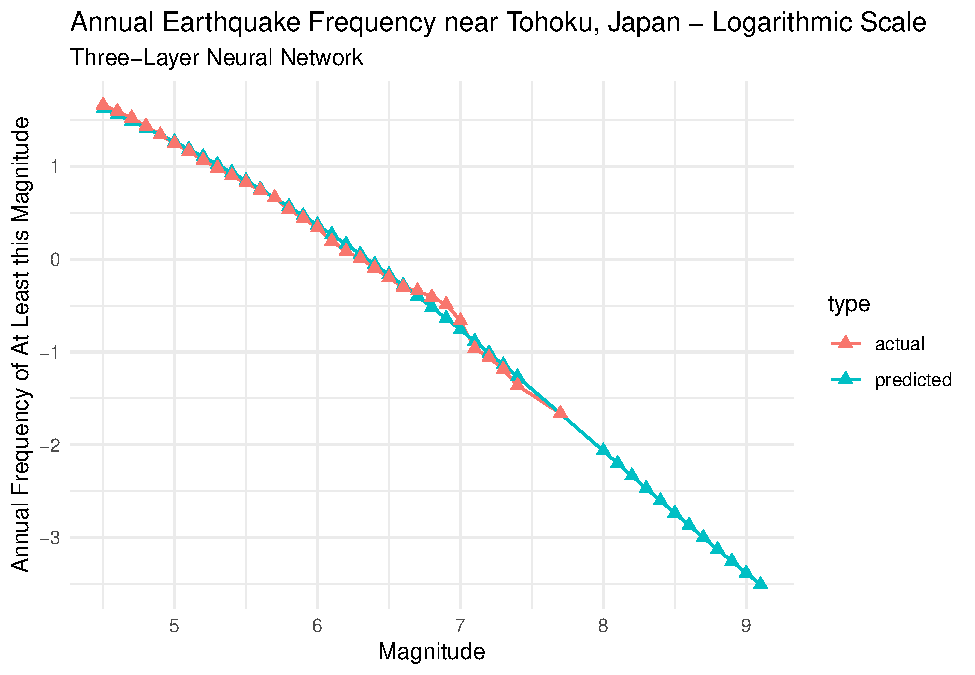
\includegraphics{earthquakes_files/figure-latex/unnamed-chunk-8-1.pdf}

\begin{Shaded}
\begin{Highlighting}[]
\CommentTok{\#{-}{-}{-}generate plot returned to the standard scale{-}{-}{-}}
\FunctionTok{ggplot}\NormalTok{(mlp\_plot, }\FunctionTok{aes}\NormalTok{(}\AttributeTok{x =}\NormalTok{ mag, }\AttributeTok{y =} \DecValTok{10}\SpecialCharTok{\^{}}\NormalTok{freqc, }\AttributeTok{group =}\NormalTok{ type, }\AttributeTok{color =}\NormalTok{ type)) }\SpecialCharTok{+}
  \FunctionTok{geom\_line}\NormalTok{() }\SpecialCharTok{+}
  \FunctionTok{geom\_point}\NormalTok{(}\AttributeTok{size =} \DecValTok{2}\NormalTok{, }\AttributeTok{shape =} \DecValTok{17}\NormalTok{ ) }\SpecialCharTok{+}
  \FunctionTok{theme\_minimal}\NormalTok{() }\SpecialCharTok{+}
  \FunctionTok{labs}\NormalTok{(}\AttributeTok{x =} \StringTok{"Magnitude"}\NormalTok{,}
       \AttributeTok{y =} \StringTok{"Annual Frequency of At Least this Magnitude"}\NormalTok{,}
       \AttributeTok{title =} \StringTok{"Annual Earthquake Frequency near Tohoku, Japan {-} Standard Scale"}\NormalTok{,}
       \AttributeTok{subtitle =} \StringTok{"Three{-}Layer Neural Network"}\NormalTok{)}
\end{Highlighting}
\end{Shaded}

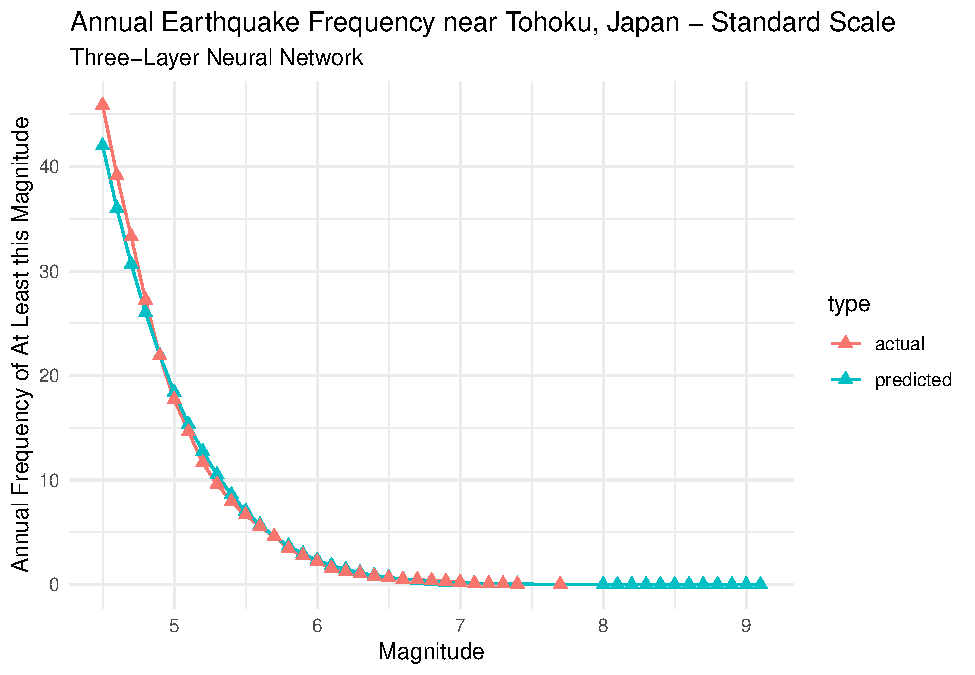
\includegraphics{earthquakes_files/figure-latex/unnamed-chunk-8-2.pdf}

\hypertarget{testing-capacity-levels-and-test-error}{%
\subsubsection{Testing Capacity Levels and Test
Error}\label{testing-capacity-levels-and-test-error}}

Three neural networks are tested, each with one more hidden layer than
the last. Each hidden layer has 5 neurons with the same architecture
otherwise.

\begin{Shaded}
\begin{Highlighting}[]
\CommentTok{\#seed must be set before each model is built}
\FunctionTok{set.seed}\NormalTok{(}\DecValTok{4723}\NormalTok{)}
\CommentTok{\#{-}{-}{-}one hidden layer{-}{-}{-}}
\NormalTok{mlp }\OtherTok{\textless{}{-}} \FunctionTok{neuralnet}\NormalTok{(freqc }\SpecialCharTok{\textasciitilde{}}\NormalTok{ mag,}
                 \AttributeTok{stepmax =} \FloatTok{1e+06}\NormalTok{,}
                 \AttributeTok{data =}\NormalTok{ train,}
                 \AttributeTok{hidden =} \FunctionTok{c}\NormalTok{(}\DecValTok{5}\NormalTok{))}

\CommentTok{\# predictions on test data and uncertainty measures}
\NormalTok{pps }\OtherTok{\textless{}{-}} \FunctionTok{predict}\NormalTok{(mlp, }\AttributeTok{newdata =} \FunctionTok{data.frame}\NormalTok{(}\AttributeTok{mag =}\NormalTok{ test}\SpecialCharTok{$}\NormalTok{mag))}
\NormalTok{TestErr1 }\OtherTok{\textless{}{-}} \FunctionTok{sum}\NormalTok{((pps }\SpecialCharTok{{-}}\NormalTok{ test}\SpecialCharTok{$}\NormalTok{freqc)}\SpecialCharTok{\^{}}\DecValTok{2}\NormalTok{) }\CommentTok{\# SSE to get test error}
\NormalTok{TrainErr1 }\OtherTok{\textless{}{-}}\NormalTok{ mlp}\SpecialCharTok{$}\NormalTok{result.matrix[}\DecValTok{1}\NormalTok{,]    }\CommentTok{\# final minimized cost function error}

\FunctionTok{set.seed}\NormalTok{(}\DecValTok{4723}\NormalTok{)}
\CommentTok{\#{-}{-}{-}two hidden layers{-}{-}{-}}
\NormalTok{mlp }\OtherTok{\textless{}{-}} \FunctionTok{neuralnet}\NormalTok{(freqc }\SpecialCharTok{\textasciitilde{}}\NormalTok{ mag,}
                 \AttributeTok{stepmax =} \FloatTok{1e+06}\NormalTok{,}
                 \AttributeTok{data =}\NormalTok{ train,}
                 \AttributeTok{hidden =} \FunctionTok{c}\NormalTok{(}\DecValTok{5}\NormalTok{,}\DecValTok{5}\NormalTok{))}

\CommentTok{\# predictions on test data and uncertainty measures}
\NormalTok{pps }\OtherTok{\textless{}{-}} \FunctionTok{predict}\NormalTok{(mlp, }\AttributeTok{newdata =} \FunctionTok{data.frame}\NormalTok{(}\AttributeTok{mag =}\NormalTok{ test}\SpecialCharTok{$}\NormalTok{mag))}
\NormalTok{TestErr2 }\OtherTok{\textless{}{-}} \FunctionTok{sum}\NormalTok{((pps }\SpecialCharTok{{-}}\NormalTok{ test}\SpecialCharTok{$}\NormalTok{freqc)}\SpecialCharTok{\^{}}\DecValTok{2}\NormalTok{) }\CommentTok{\# SSE to get test error}
\NormalTok{TrainErr2 }\OtherTok{\textless{}{-}}\NormalTok{ mlp}\SpecialCharTok{$}\NormalTok{result.matrix[}\DecValTok{1}\NormalTok{,]    }\CommentTok{\# final minimized cost function error}

\FunctionTok{set.seed}\NormalTok{(}\DecValTok{4723}\NormalTok{)}
\CommentTok{\#{-}{-}{-}three hidden layers{-}{-}{-}}
\NormalTok{mlp }\OtherTok{\textless{}{-}} \FunctionTok{neuralnet}\NormalTok{(freqc }\SpecialCharTok{\textasciitilde{}}\NormalTok{ mag,}
                 \AttributeTok{stepmax =} \FloatTok{1e+06}\NormalTok{,}
                 \AttributeTok{data =}\NormalTok{ train,}
                 \AttributeTok{hidden =} \FunctionTok{c}\NormalTok{(}\DecValTok{5}\NormalTok{,}\DecValTok{5}\NormalTok{,}\DecValTok{5}\NormalTok{))}

\CommentTok{\# predictions on test data and uncertainty measures}
\NormalTok{pps }\OtherTok{\textless{}{-}} \FunctionTok{predict}\NormalTok{(mlp, }\AttributeTok{newdata =} \FunctionTok{data.frame}\NormalTok{(}\AttributeTok{mag =}\NormalTok{ test}\SpecialCharTok{$}\NormalTok{mag))}
\NormalTok{TestErr3 }\OtherTok{\textless{}{-}} \FunctionTok{sum}\NormalTok{((pps }\SpecialCharTok{{-}}\NormalTok{ test}\SpecialCharTok{$}\NormalTok{freqc)}\SpecialCharTok{\^{}}\DecValTok{2}\NormalTok{) }\CommentTok{\# SSE to get test error}
\NormalTok{TrainErr3 }\OtherTok{\textless{}{-}}\NormalTok{ mlp}\SpecialCharTok{$}\NormalTok{result.matrix[}\DecValTok{1}\NormalTok{,]    }\CommentTok{\# final minimized cost function error}


\CommentTok{\#{-}{-}{-}View results{-}{-}{-}}
\NormalTok{TestError }\OtherTok{\textless{}{-}} \FunctionTok{cbind}\NormalTok{(TestErr1,TestErr2,TestErr3)[}\DecValTok{1}\SpecialCharTok{:}\DecValTok{3}\NormalTok{]}
\NormalTok{TrainError }\OtherTok{\textless{}{-}} \FunctionTok{cbind}\NormalTok{(TrainErr1, TrainErr2, TrainErr3)[}\DecValTok{1}\SpecialCharTok{:}\DecValTok{3}\NormalTok{]}
\NormalTok{GeneralizationGap }\OtherTok{\textless{}{-}}\NormalTok{ TrainError }\SpecialCharTok{{-}}\NormalTok{ TestError}

\FunctionTok{data.frame}\NormalTok{(}\FunctionTok{rbind}\NormalTok{(TestError,TrainError,GeneralizationGap))}
\end{Highlighting}
\end{Shaded}

\begin{verbatim}
##                            X1          X2         X3
## TestError         0.009838334 0.008655795 0.01114061
## TrainError        0.038023503 0.017808021 0.02909132
## GeneralizationGap 0.028185169 0.009152226 0.01795071
\end{verbatim}

\begin{Shaded}
\begin{Highlighting}[]
\CommentTok{\#code to produce nice table}
\CommentTok{\# data.frame(rbind(TestError,TrainError,GeneralizationGap)) \%\textgreater{}\% }
\CommentTok{\#   xtable(digits = 10)}
\end{Highlighting}
\end{Shaded}

\hypertarget{bayesian-reguarized-neural-network}{%
\subsection{Bayesian Reguarized Neural
Network}\label{bayesian-reguarized-neural-network}}

Using the \texttt{brnn} package \cite{brnn} to create a 3-layer neural
network with 6 hidden neurons. Network uses Bayesian regularization to
set parameters \(\alpha\) and \(\beta\).

\begin{Shaded}
\begin{Highlighting}[]
\NormalTok{x }\OtherTok{\textless{}{-}}\NormalTok{ eq\_log}\SpecialCharTok{$}\NormalTok{mag}
\NormalTok{y }\OtherTok{\textless{}{-}}\NormalTok{ eq\_log}\SpecialCharTok{$}\NormalTok{freqc}

\NormalTok{brnn }\OtherTok{\textless{}{-}} \FunctionTok{brnn}\NormalTok{(y}\SpecialCharTok{\textasciitilde{}}\NormalTok{x,}\AttributeTok{neurons=}\DecValTok{6}\NormalTok{)   }\CommentTok{\# build model}
\end{Highlighting}
\end{Shaded}

\begin{verbatim}
## Number of parameters (weights and biases) to estimate: 18 
## Nguyen-Widrow method
## Scaling factor= 4.2 
## gamma= 6.6054     alpha= 0.1144   beta= 865.918
\end{verbatim}

\begin{Shaded}
\begin{Highlighting}[]
\FunctionTok{summary}\NormalTok{(brnn)                 }\CommentTok{\# summary of model}
\end{Highlighting}
\end{Shaded}

\begin{verbatim}
## A Bayesian regularized neural network 
## 1 - 6 - 1 with 18 weights, biases and connection strengths
## Inputs and output were  normalized
## Training finished because  Changes in F= beta*SCE + alpha*Ew in last 3 iterations less than 0.001
\end{verbatim}

\begin{Shaded}
\begin{Highlighting}[]
\CommentTok{\#{-}{-}{-}return interval of years based on 9.1 prediction}
\NormalTok{b }\OtherTok{\textless{}{-}} \FunctionTok{predict}\NormalTok{(brnn, }\AttributeTok{newdata =} \FunctionTok{data.frame}\NormalTok{(}\AttributeTok{x =} \FloatTok{9.1}\NormalTok{))}
\DecValTok{1}\SpecialCharTok{/}\NormalTok{(}\DecValTok{10}\SpecialCharTok{\^{}}\NormalTok{b)}
\end{Highlighting}
\end{Shaded}

\begin{verbatim}
## [1] 102.8546
\end{verbatim}

\hypertarget{plots-for-brnn}{%
\subsubsection{Plots for BRNN}\label{plots-for-brnn}}

Generating plots for predicted network outputs in exactly the same
manner as before with MLP.

\begin{Shaded}
\begin{Highlighting}[]
\CommentTok{\#{-}{-}{-}actual test data{-}{-}{-}}
\NormalTok{actual\_log\_brnn }\OtherTok{\textless{}{-}}\NormalTok{ eq\_log }\SpecialCharTok{\%\textgreater{}\%} 
  \FunctionTok{mutate}\NormalTok{(}\AttributeTok{type =} \StringTok{"actual"}\NormalTok{)}

\CommentTok{\#{-}{-}{-}predicted data{-}{-}{-}}
\NormalTok{mdp }\OtherTok{\textless{}{-}} \FunctionTok{seq}\NormalTok{(}\DecValTok{8}\NormalTok{,}\FloatTok{9.1}\NormalTok{, }\AttributeTok{by =}\NormalTok{ .}\DecValTok{1}\NormalTok{) }\CommentTok{\#additional magnitude data points to add to prediction data}

\NormalTok{bnn\_preds }\OtherTok{\textless{}{-}}\NormalTok{ eq\_log}\SpecialCharTok{$}\NormalTok{mag }\SpecialCharTok{\%\textgreater{}\%} \FunctionTok{append}\NormalTok{(mdp) }\CommentTok{\#append additional magnitudes to make predictions}

\NormalTok{predicted\_log\_brnn }\OtherTok{\textless{}{-}} \FunctionTok{data.frame}\NormalTok{(}\AttributeTok{mag =}\NormalTok{ bnn\_preds,}
                             \AttributeTok{freqc =} \FunctionTok{predict}\NormalTok{(brnn, }\AttributeTok{newdata =} \FunctionTok{data.frame}\NormalTok{(}\AttributeTok{x =}\NormalTok{ bnn\_preds)),}
                             \AttributeTok{type =} \StringTok{"predicted"}\NormalTok{)}


\CommentTok{\#{-}{-}{-}combine test and predictions for plot{-}{-}{-}}
\NormalTok{brnn\_plot }\OtherTok{\textless{}{-}} \FunctionTok{rbind}\NormalTok{(predicted\_log\_brnn,actual\_log\_brnn[,}\FunctionTok{c}\NormalTok{(}\DecValTok{1}\NormalTok{,}\DecValTok{3}\NormalTok{,}\DecValTok{4}\NormalTok{)])}

\CommentTok{\#{-}{-}{-}generate plot{-}{-}{-}}
\FunctionTok{ggplot}\NormalTok{(brnn\_plot, }\FunctionTok{aes}\NormalTok{(}\AttributeTok{x =}\NormalTok{ mag, }\AttributeTok{y =}\NormalTok{ freqc, }\AttributeTok{group =}\NormalTok{ type, }\AttributeTok{color =}\NormalTok{ type)) }\SpecialCharTok{+}
  \FunctionTok{geom\_line}\NormalTok{() }\SpecialCharTok{+}
  \FunctionTok{geom\_point}\NormalTok{(}\AttributeTok{size =} \DecValTok{2}\NormalTok{, }\AttributeTok{shape =} \DecValTok{17}\NormalTok{ , }\AttributeTok{alpha =}\NormalTok{ .}\DecValTok{5}\NormalTok{) }\SpecialCharTok{+}
  \FunctionTok{theme\_minimal}\NormalTok{() }\SpecialCharTok{+}
  \FunctionTok{labs}\NormalTok{(}\AttributeTok{x =} \StringTok{"Magnitude"}\NormalTok{,}
       \AttributeTok{y =} \StringTok{"Annual Frequency of At Least this Magnitude"}\NormalTok{,}
       \AttributeTok{title =} \StringTok{"Annual Earthquake Frequency near Tohoku, Japan {-} Logarithmic Scale"}\NormalTok{,}
       \AttributeTok{subtitle =} \StringTok{"Three{-}Layer Neural Network with Bayesian Regularization"}\NormalTok{)}
\end{Highlighting}
\end{Shaded}

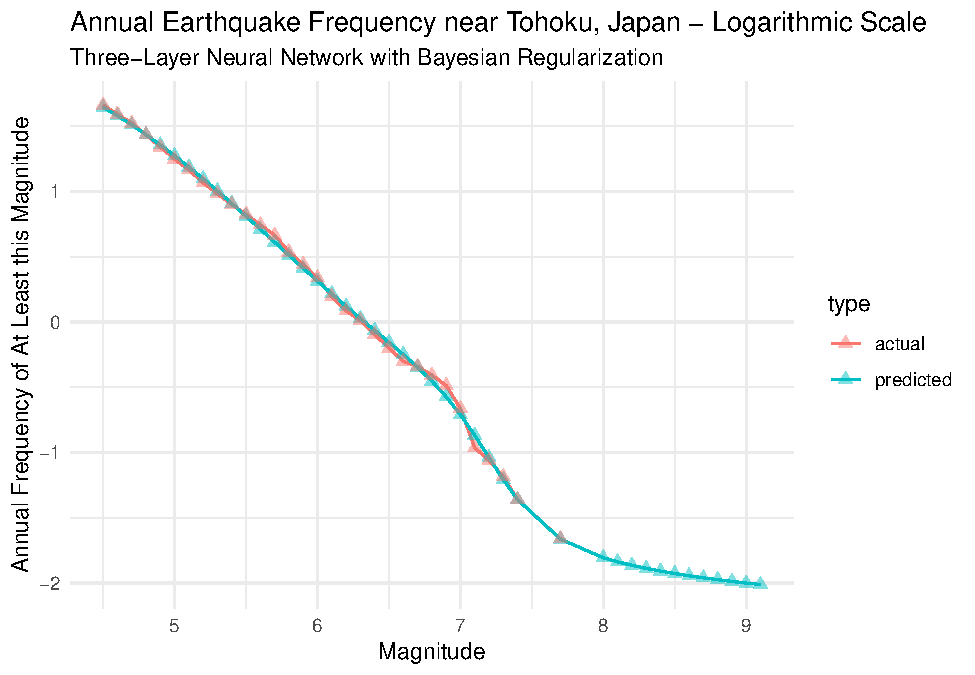
\includegraphics{earthquakes_files/figure-latex/unnamed-chunk-11-1.pdf}

\begin{Shaded}
\begin{Highlighting}[]
\CommentTok{\#{-}{-}{-}generate plot returned to the standard scale{-}{-}{-}}
\NormalTok{brnn\_plot2 }\OtherTok{\textless{}{-}}\NormalTok{ brnn\_plot }\SpecialCharTok{\%\textgreater{}\%} 
  \FunctionTok{mutate}\NormalTok{(}\AttributeTok{freqc =} \DecValTok{10}\SpecialCharTok{\^{}}\NormalTok{freqc)}

\FunctionTok{ggplot}\NormalTok{(brnn\_plot2, }\FunctionTok{aes}\NormalTok{(}\AttributeTok{x =}\NormalTok{ mag, }\AttributeTok{y =}\NormalTok{ freqc, }\AttributeTok{group =}\NormalTok{ type, }\AttributeTok{color =}\NormalTok{ type)) }\SpecialCharTok{+}
  \FunctionTok{geom\_line}\NormalTok{() }\SpecialCharTok{+}
  \FunctionTok{geom\_point}\NormalTok{(}\AttributeTok{size =} \DecValTok{2}\NormalTok{, }\AttributeTok{shape =} \DecValTok{17}\NormalTok{, }\AttributeTok{alpha =}\NormalTok{ .}\DecValTok{5}\NormalTok{) }\SpecialCharTok{+}
  \FunctionTok{theme\_minimal}\NormalTok{() }\SpecialCharTok{+}
  \FunctionTok{labs}\NormalTok{(}\AttributeTok{x =} \StringTok{"Magnitude"}\NormalTok{,}
       \AttributeTok{y =} \StringTok{"Annual Frequency of At Least this Magnitude"}\NormalTok{,}
       \AttributeTok{title =} \StringTok{"Annual Earthquake Frequency near Tohoku, Japan {-} Standard Scale"}\NormalTok{,}
       \AttributeTok{subtitle =} \StringTok{"Three{-}Layer Neural Network with Bayesian Regularization"}\NormalTok{)}
\end{Highlighting}
\end{Shaded}

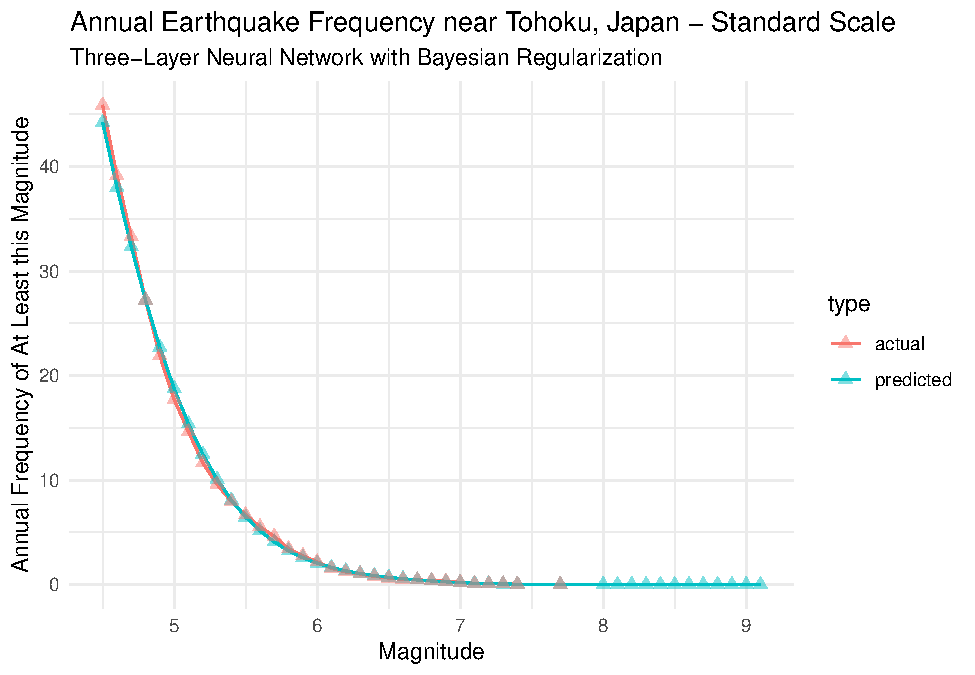
\includegraphics{earthquakes_files/figure-latex/unnamed-chunk-11-2.pdf}

\hypertarget{posterior-predictive-simulations-of-brnn---100-networks}{%
\subsection{Posterior Predictive Simulations of BRNN - 100
networks}\label{posterior-predictive-simulations-of-brnn---100-networks}}

Simulating 100 networks' predictions for relative magnitudes with
\emph{neurons = 6}.

\begin{Shaded}
\begin{Highlighting}[]
\CommentTok{\#{-}{-}{-}plot of the data predictions over actual {-} logistic scale}
\FunctionTok{ggplot}\NormalTok{(ddf, }\FunctionTok{aes}\NormalTok{(}\AttributeTok{x =}\NormalTok{ mag, }\AttributeTok{y =}\NormalTok{ freqc, }\AttributeTok{group =}\NormalTok{ iteration, }\AttributeTok{shape =}\NormalTok{ type, }\AttributeTok{alpha =}\NormalTok{ type, }\AttributeTok{color =}\NormalTok{ type)) }\SpecialCharTok{+}
  \FunctionTok{geom\_line}\NormalTok{(}\AttributeTok{show.legend =}\NormalTok{ T) }\SpecialCharTok{+}
  \FunctionTok{geom\_point}\NormalTok{(}\FunctionTok{aes}\NormalTok{(}\AttributeTok{size =}\NormalTok{ type), }\AttributeTok{shape =} \DecValTok{17}\NormalTok{) }\SpecialCharTok{+}
  \FunctionTok{theme\_minimal}\NormalTok{() }\SpecialCharTok{+}
  \FunctionTok{labs}\NormalTok{(}\AttributeTok{x =} \StringTok{"Magnitude"}\NormalTok{,}
       \AttributeTok{y =} \StringTok{"Annual Frequency of At Least this Magnitude"}\NormalTok{,}
       \AttributeTok{title =} \StringTok{"Annual Earthquake Frequency near Tohoku, Japan {-} Logarithmic Scale"}\NormalTok{,}
       \AttributeTok{subtitle =} \StringTok{"Three{-}Layer Neural Network with Bayesian Regularization"}\NormalTok{) }\SpecialCharTok{+}
  \FunctionTok{scale\_alpha\_discrete}\NormalTok{(}\AttributeTok{range =} \FunctionTok{c}\NormalTok{(}\DecValTok{1}\NormalTok{, .}\DecValTok{25}\NormalTok{)) }\SpecialCharTok{+}
  \FunctionTok{scale\_size\_discrete}\NormalTok{(}\AttributeTok{range =} \FunctionTok{c}\NormalTok{(}\DecValTok{2}\NormalTok{,}\DecValTok{1}\NormalTok{))}
\end{Highlighting}
\end{Shaded}

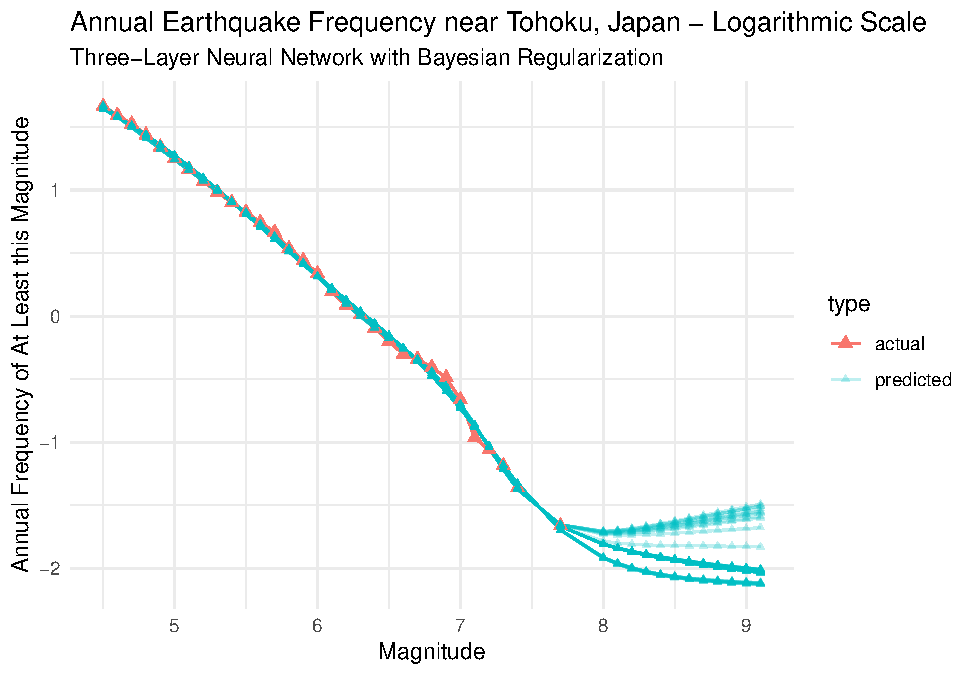
\includegraphics{earthquakes_files/figure-latex/unnamed-chunk-13-1.pdf}

\begin{Shaded}
\begin{Highlighting}[]
\CommentTok{\# subset all predictions for a 9.1}
\NormalTok{ddf\_9}\FloatTok{.1} \OtherTok{\textless{}{-}}\NormalTok{ ddf[}\FunctionTok{which}\NormalTok{(ddf}\SpecialCharTok{$}\NormalTok{mag }\SpecialCharTok{==} \FloatTok{9.1}\NormalTok{),]}

\CommentTok{\#{-}{-}{-}scatter plot of 9.1 predictions}
\FunctionTok{ggplot}\NormalTok{(ddf\_9}\FloatTok{.1}\NormalTok{, }\FunctionTok{aes}\NormalTok{(}\AttributeTok{x =}\NormalTok{ iteration, }\AttributeTok{y =} \DecValTok{1}\SpecialCharTok{/}\DecValTok{10}\SpecialCharTok{\^{}}\NormalTok{(freqc))) }\SpecialCharTok{+}
\FunctionTok{geom\_point}\NormalTok{(}\AttributeTok{size =} \DecValTok{2}\NormalTok{, }\AttributeTok{shape =} \DecValTok{16}\NormalTok{, }\AttributeTok{color =} \StringTok{"cyan4"}\NormalTok{) }\SpecialCharTok{+} 
    \FunctionTok{labs}\NormalTok{(}\AttributeTok{x =} \StringTok{"Iteration"}\NormalTok{,}
         \AttributeTok{y =} \StringTok{"Predicted Lapsed Time (Years) Between Occurrences"}\NormalTok{,}
         \AttributeTok{title =} \StringTok{"Predictions for a Magnitude 9.1 Earthquake"}\NormalTok{,}
         \AttributeTok{subtitle =} \StringTok{"Three{-}Layer Neural Network with Bayesian Regularization"}\NormalTok{) }\SpecialCharTok{+}
  \FunctionTok{theme\_minimal}\NormalTok{()}
\end{Highlighting}
\end{Shaded}

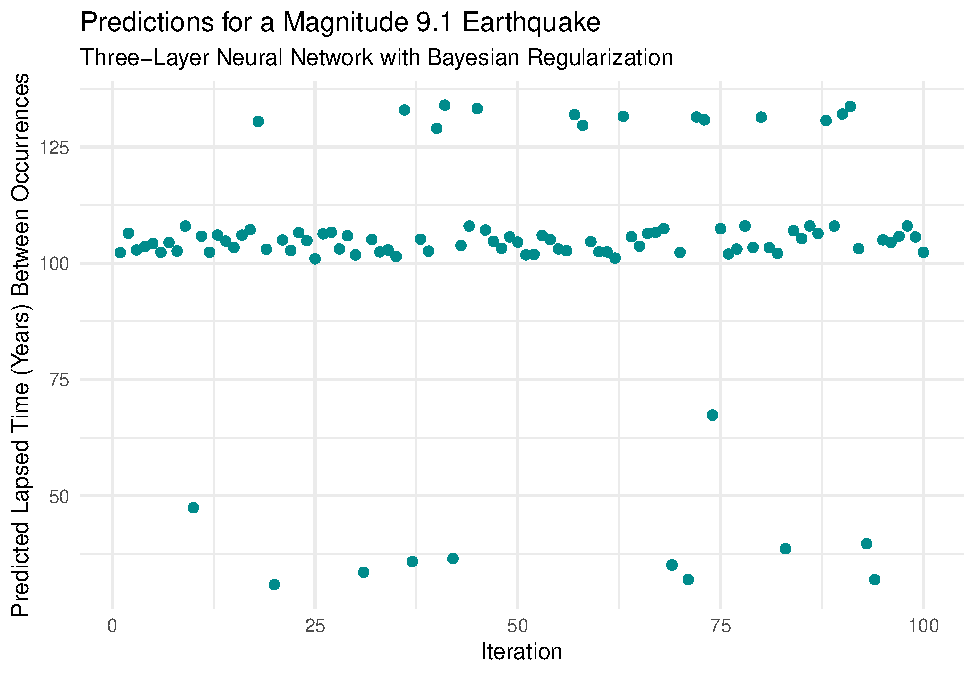
\includegraphics{earthquakes_files/figure-latex/unnamed-chunk-13-2.pdf}

\begin{Shaded}
\begin{Highlighting}[]
\CommentTok{\# delete this for Appendix}
\CommentTok{\# ggplot(ddf\_9.1, aes(sample = 1/10\^{}(freqc))) +}
\CommentTok{\# geom\_qq() + }
\CommentTok{\#     labs(x = "Iteration",}
\CommentTok{\#          y = "Predicted Lapsed Time (Years) Between Occurrences",}
\CommentTok{\#          title = "Predictions for a Magnitude 9.1 Earthquake",}
\CommentTok{\#          subtitle = "Three{-}Layer Neural Network with Bayesian Regularization") +}
\CommentTok{\#   theme\_minimal()}


\CommentTok{\#This, I believe, may just be the approximate posterior predictve distribution for a magnitude 9.1}

\CommentTok{\#{-}{-}{-}posterior predictive distribution of a magnitude 9.1}
\FunctionTok{ggplot}\NormalTok{(ddf\_9}\FloatTok{.1}\NormalTok{, }\FunctionTok{aes}\NormalTok{(}\AttributeTok{x =} \DecValTok{1}\SpecialCharTok{/}\DecValTok{10}\SpecialCharTok{\^{}}\NormalTok{(freqc))) }\SpecialCharTok{+}
\FunctionTok{geom\_density}\NormalTok{() }\SpecialCharTok{+} 
    \FunctionTok{labs}\NormalTok{(}\AttributeTok{x =} \StringTok{"Predicted Lapsed Time (Years) Between Occurrences"}\NormalTok{,}
         \AttributeTok{y =} \StringTok{"Density"}\NormalTok{,}
         \AttributeTok{title =} \StringTok{"Approximate Posterior Predictive Density of a Magnitude 9.1 Earthquake"}\NormalTok{,}
         \AttributeTok{subtitle =} \StringTok{"Three{-}Layer Neural Network with Bayesian Regularization"}\NormalTok{) }\SpecialCharTok{+}
  \FunctionTok{theme\_minimal}\NormalTok{()}
\end{Highlighting}
\end{Shaded}

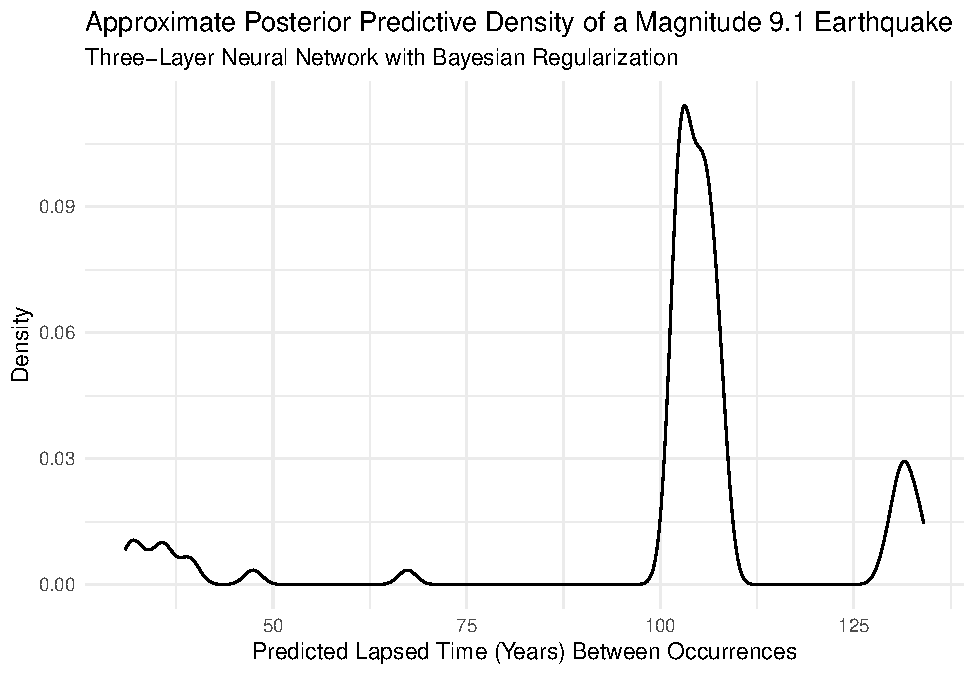
\includegraphics{earthquakes_files/figure-latex/unnamed-chunk-13-3.pdf}

\hypertarget{plots-with-outliers-removed-better-visual}{%
\subsubsection{Plots with outlier(s) removed (better
visual)}\label{plots-with-outliers-removed-better-visual}}

Visualizing 97-99\% density (contingent upon on the number of outliers
when the simulation is run) of the posterior predictive distribution.

\begin{Shaded}
\begin{Highlighting}[]
\NormalTok{ddf\_9}\FloatTok{.1}\NormalTok{\_part }\OtherTok{\textless{}{-}}\NormalTok{ ddf\_9}\FloatTok{.1}\NormalTok{[}\FunctionTok{which}\NormalTok{(ddf\_9}\FloatTok{.1}\SpecialCharTok{$}\NormalTok{freqc }\SpecialCharTok{\textgreater{}} \SpecialCharTok{{-}}\FloatTok{2.6}\NormalTok{),] }\CommentTok{\#to remove the outlier}

\CommentTok{\#{-}{-}{-}scatter plot of 9.1 predictions {-} 98{-}99\% density}
\FunctionTok{ggplot}\NormalTok{(ddf\_9}\FloatTok{.1}\NormalTok{\_part, }\FunctionTok{aes}\NormalTok{(}\AttributeTok{x =}\NormalTok{ iteration, }\AttributeTok{y =} \DecValTok{1}\SpecialCharTok{/}\DecValTok{10}\SpecialCharTok{\^{}}\NormalTok{(freqc))) }\SpecialCharTok{+}
\FunctionTok{geom\_point}\NormalTok{(}\AttributeTok{size =} \DecValTok{2}\NormalTok{, }\AttributeTok{shape =} \DecValTok{16}\NormalTok{, }\AttributeTok{color =} \StringTok{"cyan4"}\NormalTok{) }\SpecialCharTok{+} 
    \FunctionTok{labs}\NormalTok{(}\AttributeTok{x =} \StringTok{"Iteration"}\NormalTok{,}
         \AttributeTok{y =} \StringTok{"Predicted Lapsed Time (Years) Between Occurrences"}\NormalTok{,}
         \AttributeTok{title =} \StringTok{"Predictions for a Magnitude 9.1 Earthquake"}\NormalTok{,}
         \AttributeTok{subtitle =} \StringTok{"Three{-}Layer Neural Network with Bayesian Regularization"}\NormalTok{) }\SpecialCharTok{+}
  \FunctionTok{theme\_minimal}\NormalTok{()}
\end{Highlighting}
\end{Shaded}

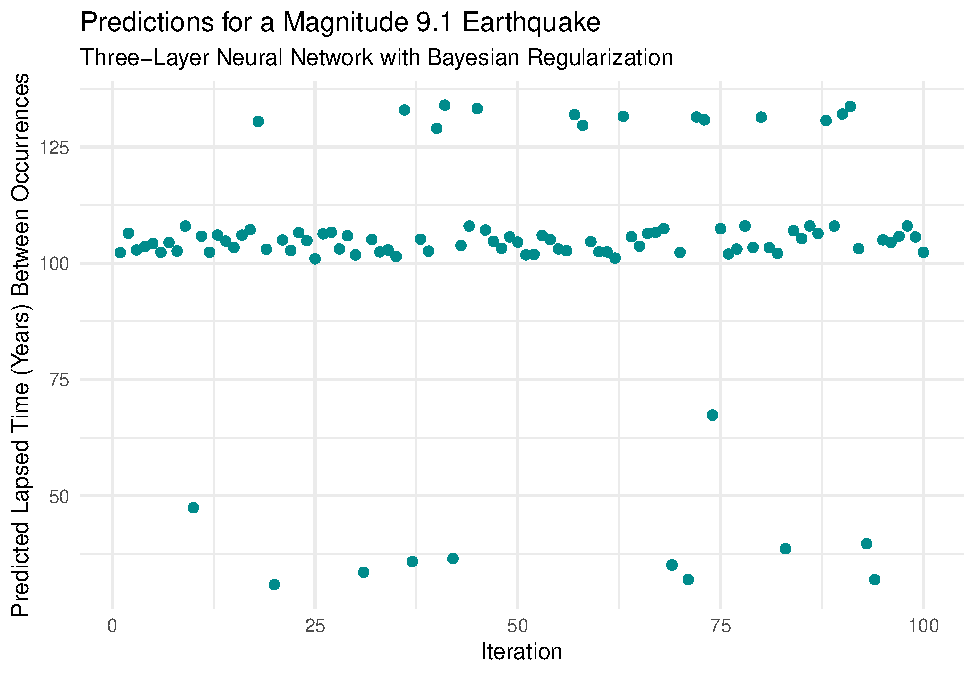
\includegraphics{earthquakes_files/figure-latex/unnamed-chunk-14-1.pdf}

\begin{Shaded}
\begin{Highlighting}[]
\CommentTok{\#{-}{-}{-}posterior predictive distribution of a 9.1 {-} 97{-}99\% density}
\FunctionTok{ggplot}\NormalTok{(ddf\_9}\FloatTok{.1}\NormalTok{\_part, }\FunctionTok{aes}\NormalTok{(}\AttributeTok{x =} \DecValTok{1}\SpecialCharTok{/}\DecValTok{10}\SpecialCharTok{\^{}}\NormalTok{(freqc))) }\SpecialCharTok{+}
\FunctionTok{geom\_density}\NormalTok{() }\SpecialCharTok{+} 
    \FunctionTok{labs}\NormalTok{(}\AttributeTok{x =} \StringTok{"Predicted Lapsed Time (Years) Between Occurrences"}\NormalTok{,}
         \AttributeTok{y =} \StringTok{"Density"}\NormalTok{,}
         \AttributeTok{title =} \StringTok{"Approximate Posterior Predictive Density of a Magnitude 9.1 Earthquake"}\NormalTok{,}
         \AttributeTok{subtitle =} \StringTok{"Three{-}Layer Neural Network with Bayesian Regularization"}\NormalTok{) }\SpecialCharTok{+}
  \FunctionTok{theme\_minimal}\NormalTok{()}
\end{Highlighting}
\end{Shaded}

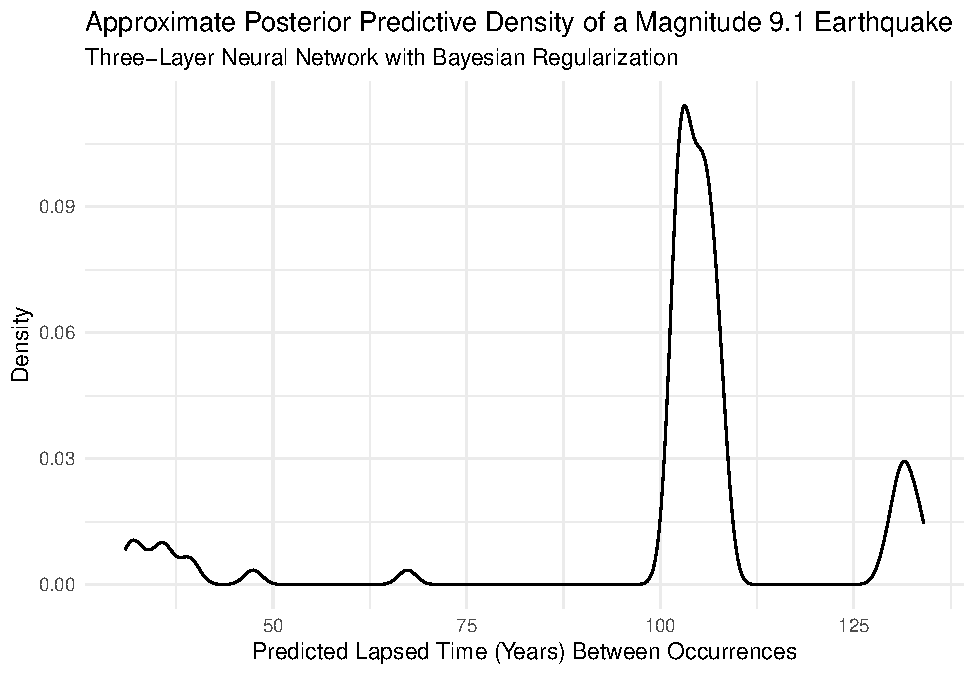
\includegraphics{earthquakes_files/figure-latex/unnamed-chunk-14-2.pdf}

\hypertarget{posterior-predictive-simulations-for-brnn---1000-networks}{%
\subsection{Posterior Predictive Simulations for BRNN - 1000
networks}\label{posterior-predictive-simulations-for-brnn---1000-networks}}

Simulating 1000 networks predictions for sharper posterior simulation

\begin{Shaded}
\begin{Highlighting}[]
\CommentTok{\# subset all predictions for a 9.1}
\NormalTok{ddf\_9}\FloatTok{.1}\NormalTok{b }\OtherTok{\textless{}{-}}\NormalTok{ ddf[}\FunctionTok{which}\NormalTok{(ddf}\SpecialCharTok{$}\NormalTok{mag }\SpecialCharTok{==} \FloatTok{9.1}\NormalTok{),]}

\CommentTok{\#{-}{-}{-}posterior predictive distribution of a 9.1 {-} full estimated density}
\FunctionTok{ggplot}\NormalTok{(ddf\_9}\FloatTok{.1}\NormalTok{b, }\FunctionTok{aes}\NormalTok{(}\AttributeTok{x =} \DecValTok{1}\SpecialCharTok{/}\DecValTok{10}\SpecialCharTok{\^{}}\NormalTok{(freqc))) }\SpecialCharTok{+}
\FunctionTok{geom\_density}\NormalTok{() }\SpecialCharTok{+} 
    \FunctionTok{labs}\NormalTok{(}\AttributeTok{x =} \StringTok{"Predicted Lapsed Time (Years) Between Occurrences"}\NormalTok{,}
         \AttributeTok{y =} \StringTok{"Density"}\NormalTok{,}
         \AttributeTok{title =} \StringTok{"Approximate Posterior Predictive Density of a Magnitude 9.1 Earthquake"}\NormalTok{,}
         \AttributeTok{subtitle =} \StringTok{"Three{-}Layer Neural Network with Bayesian Regularization"}\NormalTok{) }\SpecialCharTok{+}
  \FunctionTok{theme\_minimal}\NormalTok{()}
\end{Highlighting}
\end{Shaded}

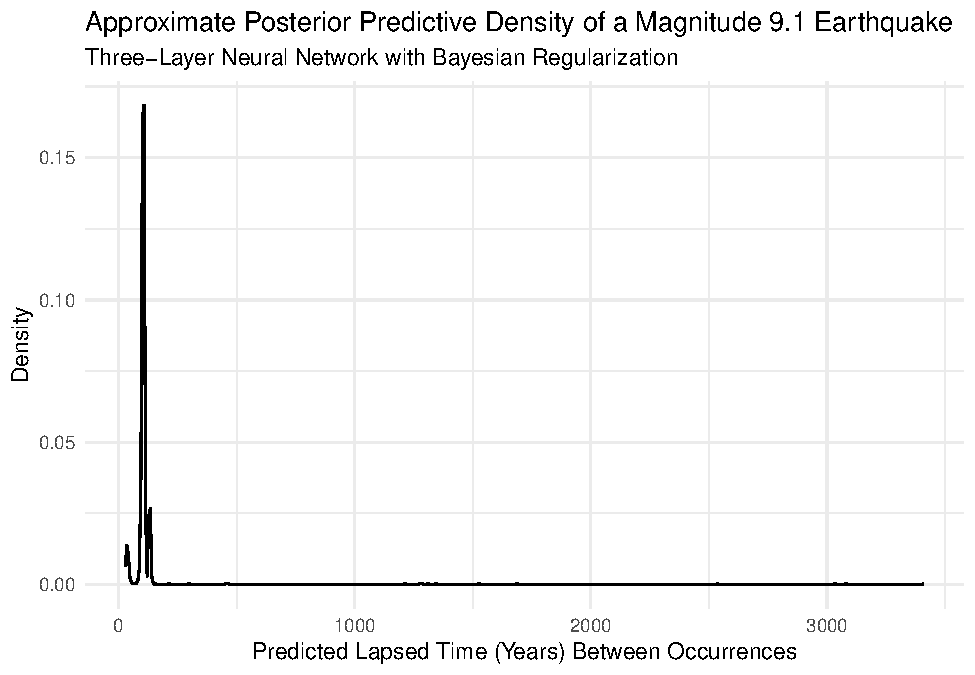
\includegraphics{earthquakes_files/figure-latex/unnamed-chunk-16-1.pdf}

\begin{Shaded}
\begin{Highlighting}[]
\NormalTok{ddf\_9}\FloatTok{.1}\NormalTok{b\_part }\OtherTok{\textless{}{-}}\NormalTok{ ddf\_9}\FloatTok{.1}\NormalTok{b[}\FunctionTok{which}\NormalTok{(ddf\_9}\FloatTok{.1}\NormalTok{b}\SpecialCharTok{$}\NormalTok{freqc }\SpecialCharTok{\textgreater{}} \SpecialCharTok{{-}}\FloatTok{2.6}\NormalTok{),] }\CommentTok{\#to remove the outlier}

\CommentTok{\#{-}{-}{-}posterior predictive distribution of a 9.1 {-} 97{-}99\% density}
\FunctionTok{ggplot}\NormalTok{(ddf\_9}\FloatTok{.1}\NormalTok{b\_part, }\FunctionTok{aes}\NormalTok{(}\AttributeTok{x =} \DecValTok{1}\SpecialCharTok{/}\DecValTok{10}\SpecialCharTok{\^{}}\NormalTok{(freqc))) }\SpecialCharTok{+}
\FunctionTok{geom\_density}\NormalTok{() }\SpecialCharTok{+} 
    \FunctionTok{labs}\NormalTok{(}\AttributeTok{x =} \StringTok{"Predicted Lapsed Time (Years) Between Occurrences"}\NormalTok{,}
         \AttributeTok{y =} \StringTok{"Density"}\NormalTok{,}
         \AttributeTok{title =} \StringTok{"Approximate Posterior Predictive Density of a Magnitude 9.1 Earthquake"}\NormalTok{,}
         \AttributeTok{subtitle =} \StringTok{"Three{-}Layer Neural Network with Bayesian Regularization"}\NormalTok{) }\SpecialCharTok{+}
  \FunctionTok{theme\_minimal}\NormalTok{()}
\end{Highlighting}
\end{Shaded}

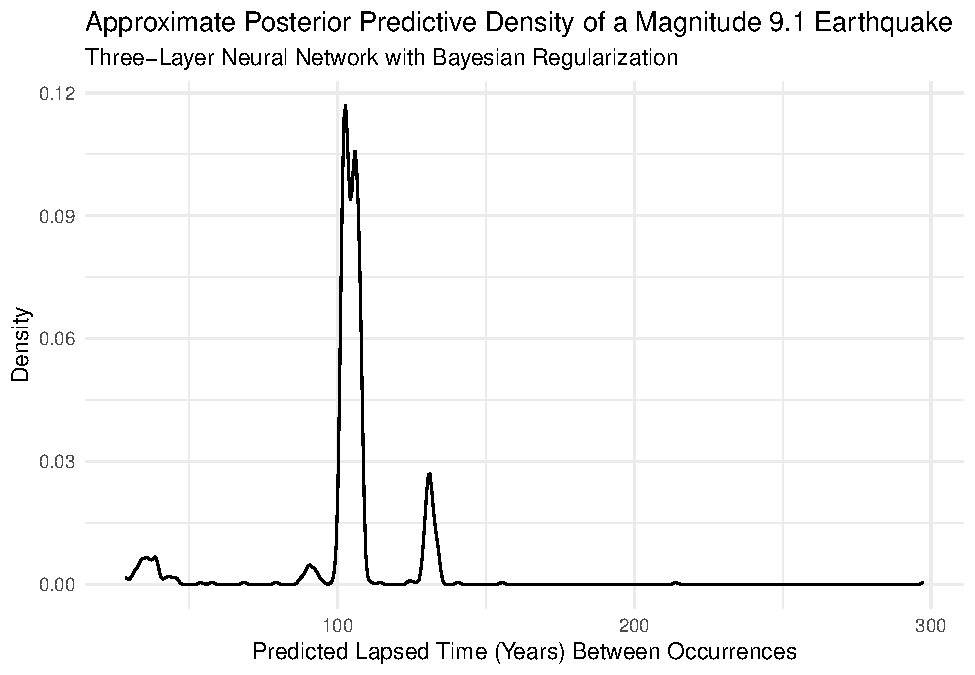
\includegraphics{earthquakes_files/figure-latex/unnamed-chunk-16-2.pdf}

